% To predlogo lahko spremeniš v PDF dokument s pomočjo programa
% pdflatex, ki je del standardne instalacije LaTeX programov.

\documentclass[a4paper,11pt]{article}
\usepackage{a4wide}
\usepackage{fullpage}
\usepackage[utf8x]{inputenc}
\usepackage[slovene]{babel}
\selectlanguage{slovene}
\usepackage[toc,page]{appendix}
\usepackage[pdftex]{graphicx} % za slike
\usepackage{setspace}
\usepackage{color}
\definecolor{light-gray}{gray}{0.95}
\usepackage{listings} % za vključevanje kode
\usepackage{hyperref}
\usepackage{amssymb}

% Matlab code
\definecolor{mygreen}{RGB}{28,172,0} % color values Red, Green, Blue
\definecolor{mylilas}{RGB}{170,55,241}

\usepackage{amsmath}
\usepackage{siunitx}
\usepackage{eurosym}

\renewcommand{\baselinestretch}{1.2} % za boljšo berljivost večji razmak
\renewcommand{\appendixpagename}{Priloge}

\lstset{ % nastavitve za izpis kode, sem lahko tudi kaj dodaš/spremeniš
language=Python,
basicstyle=\footnotesize,
basicstyle=\ttfamily\footnotesize\setstretch{1},
backgroundcolor=\color{light-gray},
}

\lstset{language=Matlab,
    %basicstyle=\color{red},
    breaklines=true,%
    morekeywords={matlab2tikz},
    keywordstyle=\color{blue},%
    morekeywords=[2]{1}, keywordstyle=[2]{\color{black}},
    identifierstyle=\color{black},%
    stringstyle=\color{mylilas},
    commentstyle=\color{mygreen},%
    showstringspaces=false,%without this there will be a symbol in the places where there is a space
    numbers=left,%
    numberstyle={\tiny \color{black}},% size of the numbers
    numbersep=9pt, % this defines how far the numbers are from the text
    emph=[1]{for,end,break},emphstyle=[1]\color{red}, %some words to emphasise
    %emph=[2]{word1,word2}, emphstyle=[2]{style},    
}


\title{Rešene izpitne naloge \\ 
	\large Optimizacijske Metode 2020/21}
\author{David Rubin}
\date{\today}

\begin{document}

\maketitle

\tableofcontents
\newpage


\section{Uvod}

Dokument predstavlja zapisnik dela, ki se je izvajalo na vajah predmeta. Poleg tega dokumenta so dostopne tudi podmape, v katerih se nahajajo \texttt{m file}, ki vsebujejo nekatere definicije za izvedbo ukazov, ki pripeljejo do ustreznih rešitev.

\section{Splošni napotki vaj}

V kolikor uporabljaš simbolične funkcije, je potrebno spremenljivke inicializirati s \texttt{syms}. V kolikor bi si rad izrisal neko funkcijo, to storiš najlažje tako, da si definiraš simbolične spremenljivke s \texttt{syms}, definiraš neko funkcijo in kličeš izris s \texttt{ezmesh} (ali \texttt{fmesh}). Malo je treba tudi ugibati pri definiciji intervala, na katerem je izris, da dobiš dobro predstavitev. Glej kodo~\ref{vaje1splosno}

\lstinputlisting[label=vaje1splosno,caption=Splošna uporaba Matlab na 1. vajah,language=Matlab]{vaje/vaje1.m}

Še nekaj koristnih napotkov pri uporabi funkcij:
\begin{itemize}
	\item \texttt{fminsearch(@($x$) function($x$), $x_0$)} ... Uporabimo, ko iščemo minimume funkcij. \texttt{@($x$)} nam pove, da je $x$ neodvisna spremenljivka. \texttt{function($x$)} je definicija neke funkcije (v večini primerov skozi ta dokument, bo ta funkcija shranjena v ločenem m-file). $x_0$ nam določa, kje bo postopek pričel, torej našo začetno točko. Priporočljivo je, da se uporabijo različne točke, saj se lahko nekatere \textit{ujamejo} v lokalne minimume, mi pa si želimo poiskati globalnega. Dovolj dobro je, da vzamemo kar nekaj naključno generiranih točk, si shranimo rešitve za vsak klic in jih med sabo primerjamo. Če so vse vrednosti enake, potem to tipično pomeni, da je algoritem našel globalni minimum v vseh primerih, rešitev je potem katerakoli izmed pridobljenih. V kolikor niso vse rešitve enake, pa vzamemo najmanjšo vrednost, saj je tam globalni minimum. Za iskanje maksimumov lahko uporabimo isto funkcijo in ji spremenimo le parametre: \texttt{fminsearch(@($x$) -function($x$), $x_0$)} (dodali smo -). Paziti je potrebno, da ima tudi rezultat potem spremenjen (negativen) predznak.
	
	\item \texttt{fmincon(@($x$) function($x$), $x_0$, $A$, $b$, $A_{eq}$, $b_{eq}$, LB, UB, NONLCON)} ... pa je funkcija, kjer išemo minimume ob podanih omejitvah. Enako kot prej sta defirnirani \texttt{function($x$)} in $x_0$, dodajo pa se še naslednji členi. Matrika $A$ predstavlja omejitve, pri katerih gre za relacijo $\leq$. V matriko $A$ zapišemo števila na levi strani pred spremenljivkami, paziti pa je potrebno, da če katera spremenljivka ni označena v omejitvi jo v matriki predstavimo s členom 0. Vektor $b$ predstavlja desno stran omejitev (torej vrednosti ki so na desni strani relacije $leq$). V kolikor je relacija $\geq$ je potrebno vse člene ustrezno pomnožiti z $-1$. Matrika $A_{eq}$ in vektor $b_{eq}$ predstavljata omejitve kjer je relacija $=$. \texttt{LB} in \texttt{UB} predstavljata spodnjo (\textit{Lower Bound}) in zgornjo mejo (\textit{Upper Bound}). \texttt{NONLCON} pa uporabimo kadar omejitve niso linearne (\textit{non linear constraints)}. V tem primeru se tipično definirajo v ločenem \textit{m-file}. Glej primer na nalogi~\ref{task:maj2008_3} ali nalogi~\ref{task:februar2014_2}.
	
\end{itemize}

Poglejmo si primer iskanja minimuma za funkcijo \texttt{bana} definirano v ločenem \textit{m-file}:
\lstinputlisting[label=minsearch_sample_function,language=Matlab]{vaje/bana.m}
Uporabimo klic in določimo nek interval (pri tem lahko za enostavne funkcije pomaga izris):
\begin{lstlisting}[label=minsearch_sample_call,language=Matlab]
% Funkcija vraca tocko x, vrednost minimuma fval, in zastavico flag (katero opazujemo da je 1 - pomeni da je najdena ustrezna resitev)
[x, fval, flag] = fminsearch(@(x)bana(x), [-3, -3])
% Vrne:
%	x =[-2.7468   -2.7468]
%	fval = -100.1178
%	flag = 1
% Imamo se en lokalni minimum, ce ponovimo iskanje v drugi tocki
[x, fval, flag] = fminsearch(@(x)bana(x), [-3, 3])
% Vrne:
%	x =[-2.7468   2.9035]
%	fval = -128.3912
%	flag = 1
\end{lstlisting}


\section{Izpitne naloge}

V nadaljevanju sledijo izpitne naloge in postopki za pridobitev rešitev.
\newpage

\subsection{Izpit 23. maj 2008}

\subsubsection{Naloga 1.)}
\label{task:maj2008_1}

\textbf{Navodila:} \\ 
Minimiziraj funkcijo:

\begin{equation} \label{eq:maj2008_1}
f(x) = (x_1 - 0.5)^2 (x_1 + 1)^2 + (x_2 + 1)^2 (x_2 - 1)
\end{equation}
Ali ima funkcija samo en lokalni minimum oziroma maksimum? Če jih ima morda več, jih poišči! Kolikšna je vrednost funkcije v točki minimuma. Pomagaš si lahko z risanjem funkcije.

\vspace{5mm}
\noindent \textbf{Rešitev:} \\ 
Funkcijo si lahko izrišemo s pomočjo ukazov

\begin{lstlisting}[language=Matlab]
syms x y
f = (x - 0.5)^2 * (x + 1)^2 + (y + 1)^2 * (y - 1)^2;
fmesh(f, [-3, 3])
\end{lstlisting}
V novem \texttt{maj2008\_1.m} si definiramo funkcijo:
\lstinputlisting[language=Matlab]{exams/maj2008_1.m}
Potem lahko napišemo skripto (oziroma preverimo v zanki) iskanje minimuma iz večih točk:

\begin{lstlisting}[language=Matlab]
resitve = [];  % vnaprej pripravljen vektor resitev
for i=1:100  % 100 iteracij
	random_x0 = 20 * rand(1:2) - 10  % nakljucna zacetna tocka iz intervala [-10, 10]
	[x, fval, flag] = fminsearch(@(x)maj2008_1(x), random_x0)
	if flag == 1
		resitve = [resitve; [x fval]]  % shrani si dobre resitve
	end
end
b = uniquetol(resitve, 1e-6, 'byrows', true)  % izloci duplikatne resitve
% Vrne v stilu:
% b = 
%    -1.00  -1.00  0
%    -1.00   1.00  0
%     0.50   1.00  0
%     0.50  -1.00  0
\end{lstlisting}
Te unikatne rešitve so potem vrednosti za naše minimume. Prva dva stolpca sta vrednosti $x_1$ in $x_2$, tretji stolpec pa vrednost funkcije v tej točki $f(x_1, x_2)$.
Za iskanje maksimuma vidimo na grafu da je samo 1 in se nahaja v bližini točke $[0, 0]$, zato uporabimo le 1 klic:

\begin{lstlisting}
[x, fval, flag] = fminsearch(@(x)-maj2008_1(x), [0, 0])
% Vrne v stilu:
% x = [-0.2500    0.0000]
% fval = -1.3164
% flag = 1
\end{lstlisting}
Kar pomeni da je točka $[-0.25, 0]$ lokalni maksimum z vrednostjo -1.3164.


\subsubsection{Naloga 2.)}
\label{task:maj2008_2}

\textbf{Navodila:} \\
Maksimiziraj funkcijo in izračunaj njeno vrednost v točki maksimuma:
\begin{equation} \label{eq:maj2008_2}
f(x) = (x_1^2 + 2x_2^2)e^{-(x_1^2 + x_2^2)}
\end{equation}
\textbf{Rešitev:} \\
Podobno kot v nalogi~\ref{task:maj2008_1} si najprej narišemo funkcijo, in potem poskušamo identificirati število in postopek iskanja maksimumov:

\begin{lstlisting}[language=Matlab]
syms x y
f = (x^2 + 2*y^2) * exp( -(x^2 + y^2) );
fmesh(f, [-3, 3])
\end{lstlisting}

\begin{figure}[hbt]
\centering
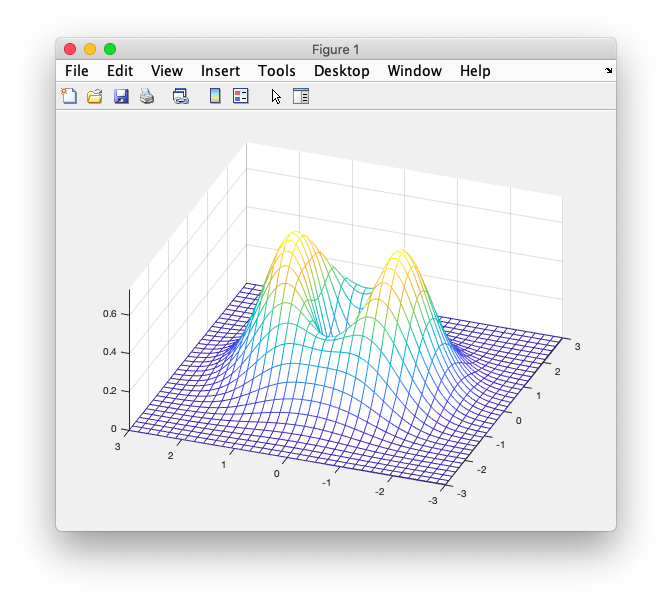
\includegraphics[scale=.4]{images/nal2_maj2008_plot.png}
\caption{Izris funkcije~\ref{eq:maj2008_2} na intervalu $[-3, 3]$.}
\label{img:maj2008_2_plot}
\end{figure}

Pri izrisu (glej sliko~\ref{img:maj2008_2_plot}) vidimo, da ima funkcija 2 vrhova in to v bližini točk $[0, -1]$ in $[0, 1]$. Funkcijo definiramo v ločenem \textit{m-file} (\texttt{maj2008\_2.m}):
\lstinputlisting[language=Matlab]{exams/maj2008_2.m} 
... in uporabimo informacijo iz izrisa v naslednjem klicu:
\begin{lstlisting}
[x, fval, flag] = fminsearch(@(x)-maj2008_2(x), [0, 1])
% Vrne v stilu:
% x =  [0    1]
% fval = -0.7358
% flag = 1
[x, fval, flag] = fminsearch(@(x)-maj2008_2(x), [0, -1])
% Vrne v stilu:
% x =  [0   -1]
% fval = -0.7358
% flag = 1
\end{lstlisting}
Točke, ki smo jih ocenili na grafu, so očitno maksimumi. Treba pa je paziti, saj je vrednost maksimumov v \texttt{fval} obratna - pravina vrednost obeh maksimumov je torej $f_{max} = 0.7358$.


\subsubsection{Naloga 3.)}
\label{task:maj2008_3}

\textbf{Navodila:} \\
Določi minimum funkcije in njeno vrednost v točki minimuma:
\begin{equation} \label{eq:maj2008_3}
f(x) = (x_1 - 2)^2 + (x_2 - 1)^2
\end{equation}
ob naslednjih omejitvah
\begin{equation} \label{con:maj2008_3}
\begin{aligned}
-x_1 -x_2 + 2 \geq 0 \\
-x_1^2 + x_2 \geq 0
\end{aligned}
\end{equation}
\textbf{Rešitev:} \\
Najprej si izrišimo funkcijo, da dobimo vpogled s čem imamo opravka (glej sliko~\ref{img:maj2008_3_plot}). Vidimo, da imamo 1 globalni minimum nekje relativno blizu točke $[0, 0]$.

\begin{figure}[hbt]
\centering
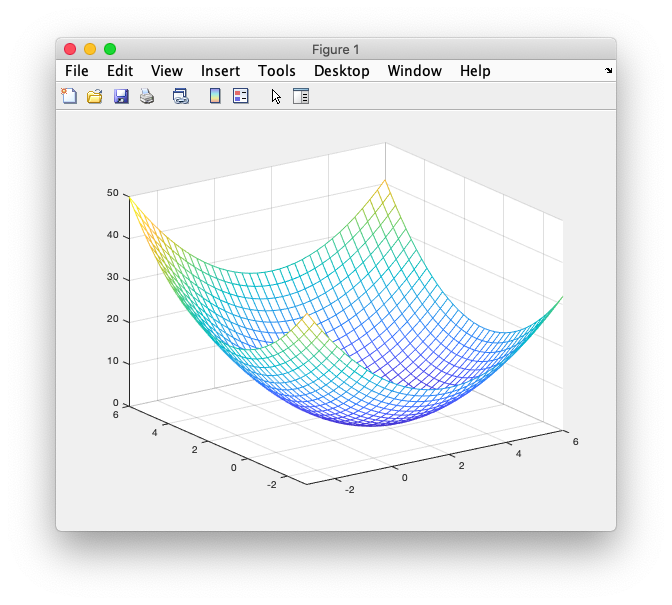
\includegraphics[scale=.4]{images/maj2008_3_plot.png}
\caption{Izris funkcije~\ref{eq:maj2008_3} na intervalu $[-3, 6]$.}
\label{img:maj2008_3_plot}
\end{figure}

V ločenem \textit{m-file} si sedaj definiramo funkcijo (\texttt{maj2008\_3.m}):
\lstinputlisting[language=Matlab]{exams/maj2008_3.m}
... in omejitve (\texttt{maj2008\_3\_con.m}):
\lstinputlisting[language=Matlab]{exams/maj2008_3_con.m}
Omejitve so tipa $\geq$, zato smo jih pomnožili s $-1$ preden smo jih vstavili v spremenljvko \texttt{c}. Sedaj lahko poženemo iskanje minimuma v bližini $[0, 0]$:
\begin{lstlisting}
[x, fval, flag] = fmincon(@(x)maj2008_3(x), [0, 0], [], [], [], [], [], [], @(x)maj2008_3_con(x))
% Vrne v stilu:
% x =  [1.000   -1.000]
% fval = 1.0000
% flag = 1
\end{lstlisting}
kar nam vrne rešitev $f_{min} = 1.000$ v točki $[1, -1]$.


\subsubsection{Naloga 4.)}
\label{task:maj2008_4}

\textbf{Navodila:} \\
Poišči vse ničle enačbe:
\begin{equation} \label{eq:maj2008_4}
f(x) = x^5 -6x^4 - 92x^3 + 402x^2 + 91x - 396
\end{equation}
\textbf{Rešitev:} \\
Uporabimo funkcijo \texttt{roots} in ji podamo koeficiente za vsako stopnjo $x$:
\begin{lstlisting}
roots([1 -6 -92 402 91 -396])
% Vrne v stilu:
% ans =
%    -9.0000
%    11.0000
%     4.0000
%    -1.0000
%     1.0000
\end{lstlisting}
Rešitev (ničle) so torej pri $x \in \{-9, -1, 1, 4, 11\}$


\subsubsection{Naloga 5.)}
\label{task:maj2008_5}

\textbf{Navodila:} \\
Letalska družba kupuje gorivo za letala pri treh različnih prodajalcih. Družba potrebuje v naslednjem mesecu na vsakem od treh letališč, kjer pristaja, naslednje količine goriva: $100.000 \si{\litre}$  na letališču 1, $180.000 \si{\litre}$ na letališču 2 ter $350.000 \si{\litre}$ na letališču 3. Gorivo prodajajo trije prodajalci, njihovo ceno goriva na posameznem letališču podaja naslednja tabela (cene so v centih na liter):
\begin{table}[hbt]
 	\centering
	\begin{tabular}{| l | c | c | c | }
		\hline
 			& Letališče 1 & Letališče 2  & Letališče 3 \\ \hline
		Prodajalec 1 & 92 & 89 & 90 \\ \hline
		Prodajalec 2 & 91 & 91 & 95 \\ \hline
		Prodajalec 3 & 87 & 90 & 92 \\ \hline
	\end{tabular}
\end{table}

Vsak prodajalec pa ima na voljo omejene količine goriva, ki ga skupno lahko dostavi v posameznem mesecu. Te količine so $320.000\si{\litre}$ prvi prodajalec, $270.000\si{\litre}$ drugi ter $190.000\si{\litre}$  tretji prodajalec. Določi pravilo za nakup goriva letalske družbe, ki bo zadovoljilo njihovim potrebam na vsakem od letališč ter bo ekonomsko čimbolj ugodno.

\vspace{5mm}
\noindent \textbf{Rešitev}: \\
Najprej si zastavimo spremenljivke $x_i,$ kjer  $i  \in \{1, 2, 3, 4, 5, 6, 7, 8, 9\}$, pri čemer je $x_1$ količina goriva kupljenega na letališču 1 pri prodajalcu 1, $x_2$ je količina goriva kupljenega na letališču 2 pri prodajalcu 1, ... in $x_9$ je količina goriva kupljenega na letališču 3 pri prodajalcu 3. Iz tega sledijo omejitve:

\begin{equation} \label{con:maj2008_5}
\begin{gathered}
x_1 + x_2 + x_3 \geq 320.000 \\
x_4 + x_5 + x_6 \geq 270.000 \\
x_7 + x_8 + x_9 \geq 190.000 \\
x_1 + x_4 + x_7 = 100.000 \\
x_2 + x_5 + x_8 = 180.000 \\
x_3 + x_6 + x_9 = 350.000 \\
x_1, x_2, x_3, x_4, x_5, x_6, x_7, x_8, x_9 \geq 0
\end{gathered}
\end{equation}
... in funkcija, ki jo minimiziramo:
\begin{equation} \label{eq:maj2008_5}
f(x) = 92x_1 + 89x_2 + 90x_3 + 91x_4 + 91x_5 + 95x_6 + 87x_7 + 90x_8 + 92x_9
\end{equation}
Vključili smo tudi omejitev nenegativnosti, saj smatramo, da letalska družba ne želi preprodajati goriva iz enega letališča na drugo (torej kupiti negativno količino). Problem lahko rešimo s funkcijo \texttt{intlinprog}:
\lstinputlisting[language=Matlab]{exams/maj2008_5.m}
Iz tega lahko razberemo, da je najugodneje na letališu 1 kupiti $100.000\si{\litre}$ pri prodajalcu 3, na letališču 2 $120.000\si{\litre}$ pri prodajalcu 2 in $60.000\si{\litre}$ pri prodajalcu 3, na letališču 3 pa $320.000\si{\litre}$ pri prodajalcu 1 in $30.000\si{\litre}$ pri prodajalcu 3. Skupno bomo porabili 565.800,00 \euro{}.


\subsection{Izpit 11. junij 2008}

\subsubsection{Naloga 1.)}
\label{task:junij2008_1}

\textbf{Navodila:} \\
Poišči vse lokalne ekstreme funkcije na intervalu $[-3, 3]$ in njene vrednosti v teh točkah:
\begin{equation} \label{eq:junij2008_1}
f(x) = \frac{1}{2}( \sin(5x) - x)^2
\end{equation}
\textbf{Rešitev:} \\
Izrišimo funkcijo:

\begin{figure}[hbt]
\centering
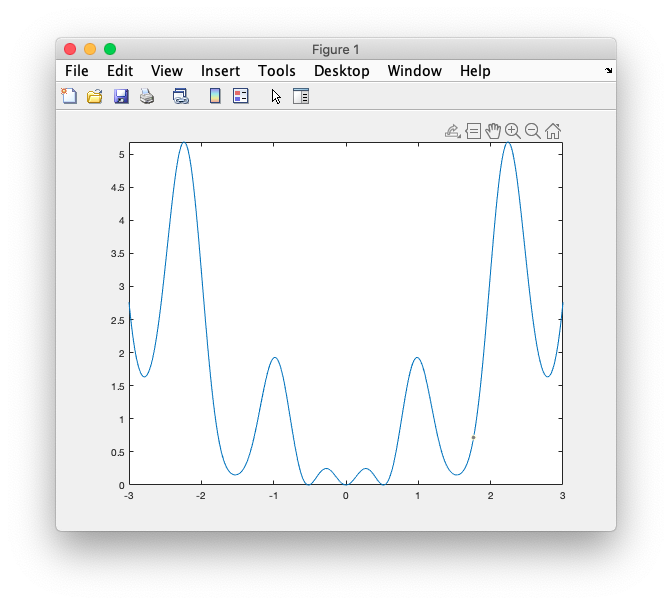
\includegraphics[scale=.4]{images/junij2008_1_plot.png}
\caption{Izris funkcije~\ref{eq:junij2008_1} na intervalu $[-3, 3]$.}
\label{img:junij2008_1_plot}
\end{figure}
Vidimo, da imamo 7 lokalnih minimumov in 6 lokalnih maksimumov. \textbf{TODO}


\subsubsection{Naloga 2.)}
\label{task:junij2008_2}

\textbf{Navodila:} \\
Reši naslednji sistem enačb:
\begin{equation} \label{eq:junij2008_2}
	\begin{gathered}
		\sin(x + y) = 0 \\
		\cos(x - y) = 0
	\end{gathered}
\end{equation}
\textbf{Rešitev:} \\
V novem \textit{m-file} si definiramo enačbi (\texttt{junij2008\_2.m}):
\lstinputlisting[language=Matlab]{exams/junij2008_2.m}
... in nato kličemo funkcijo \texttt{fsolve}:
\begin{lstlisting}[language=Matlab]
% Poskusimo najprej s [0, 0]
x = fsolve(@(x)junij2008_2(x), [0, 0])
% Kar vrne, da ni resitve ...
% Premaknimo se v negativni del
xL = fsolve(@(x)junij2008_2(x), [-.5, -.5])
% ... in v pozitivni
xR = fsolve(@(x)junij2008_2(x), [.5, .5])
% In dobimo najmanjsi resitvi (ostale so periodicne)
% xL = 	[0.7854    -0.7854]
% xR =  [-0.7854    0.7854]
\end{lstlisting}
Rešitev so torej točke $x_1 = \frac{\pi}{4}$, $y_1 = -\frac{\pi}{4}$ in $x_2 = -\frac{\pi}{4}$, $y_2 = \frac{\pi}{4}$. Rešitve se periodično ponavljajo vsake $\frac{\pi}{2}$.

\subsubsection{Naloga 3.)}
\label{task:junij2008_3}

\textbf{Navodila:} \\
Določi minimum funkcije in njeno vrednost v točki minimuma:
\begin{equation} \label{eq:junij2008_3}
f(x) = x_1^2 + 5x_2^2 + 10x_3^2 - 4x_1x_2 + 6x_1x_3 - 12x_2x_3 - 2x_1 + 10x_2 - 5x_3
\end{equation}
ob naslednjih omejitvah:
\begin{equation} \label{con:junij2008_3}
	\begin{gathered}
		x_1 + 2x_2 + x_3 \geq 4 \\
		x_1, x_2, x_3 \geq 0
	\end{gathered}
\end{equation}
\textbf{Rešitev:} \\
V novem \textit{m-file} si definiramo funkcijo (\texttt{junij2008\_3.m}):
\lstinputlisting[language=Matlab]{exams/junij2008_3.m}
In kličemo funkcijo \texttt{fmincon}:
\begin{lstlisting}[language=Matlab]
[x, fval] = fmincon(@(x)junij2008_3(x), [1 1 1], [-1 -2 -1], -4, [], [], [0 0 0])
% Vrne v stilu:
% x = [2.9412    0.5294    0.0000]
% fval = 3.2353
\end{lstlisting}
Začnemo v naključni točki $[1, 1, 1]$, omejitve (matrika $A$ in vektor $b$) morajo upoštevati relacijo $\leq$, zato so vrednosti obratne, $A_{eq}$ in $b_{eq}$ pustimo prazne, nastavimo pa še spodnjo mejo z $[0, 0, 0]$.
Rešitev je torej točka $x_{min} = [2.9412, 0.5294, 0.0000]$, v kateri imamo vrednost $f(x_{min}) = 3.2353$


\subsubsection{Naloga 4.)}
\label{task:junij2008_4}

\textbf{Navodila:} \\
Poišči minimum funkcije in njeno funkcijsko vrednost v točki minimuma:
\begin{equation} \label{eq:junij2008_4}
	f(x) = 2x_1^2 - x_1x_2 + x_2^2 - 3x_1 + e^{2x_1 + x_2}
\end{equation}
\textbf{Rešitev:} \\
Ker imamo le 2 spremenljivki, si izrišimo funkcijo (glej sliko~\ref{img:junij2008_4_plot}). 

\begin{figure}[hbt]
	\centering
	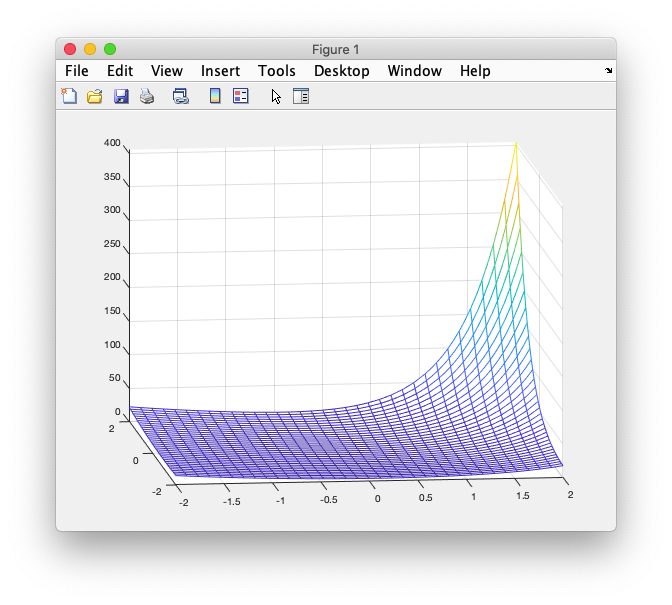
\includegraphics[scale=.4]{images/junij2008_4_plot.png}
	\caption{Izris funkcije~\ref{eq:junij2008_4} na intervalu $[-2, 2]$.}
	\label{img:junij2008_4_plot}
\end{figure}
Vidimo, da je nekje v bližini točke $[0, 0]$ morda minimum. Deifinirajmo nov \textit{m-file} (\texttt{junij2008\_4.m}):
\lstinputlisting[language=Matlab]{exams/junij2008_4.m}
... in kličemo funkcijo \texttt{fminsearch}:

\begin{lstlisting}[language=Matlab]
[x, fval, flag] = fminsearch(@(x)junij2008_4(x), [0, 0])
% Vrne v stilu:
% x = [0.1737   -0.3915]
% fval = 0.7174
% flag = 1
\end{lstlisting}
... ki nam poda našo rešitev: $x_{min} =  [0.1737, -0.3915]$, $f(x_{min}) = 0.7174$.

\subsubsection{Naloga 5.)}
\label{task:junij2008_5}

\textbf{Navodilo:} \\
Trgovina z malimi živalmi je ugotovila, da potrebuje hrček najmanj 70 enot beljakovin, 100 enot ogljikovih hidratov ter 20 enot maščob dnevno. Trgovina ima na zalogi 6 različnih vrst hrane za hrčke z naslednjimi lastnostmi:
\begin{table}[h]
	\centering
	\begin{tabular}{| c | c | c | c | c |}
		\hline
		Hrana & Beljakovin/dozo & Ogljikovih hidratov/dozo & Maščob / dozo & Cena / dozo \\ \hline
		A & 20 & 50 & 4 & 2 \\ \hline
		B & 30 & 30 & 9 & 3 \\ \hline
		C & 40 & 20 & 11 & 5 \\ \hline
		D & 40 & 25 & 10 & 6 \\ \hline
		E & 45  & 50 & 9 & 8 \\ \hline
		F & 30 & 20 & 10 & 8 \\ \hline
	\end{tabular}
\end{table}
Kakšno razmerje posameznih vrst hrane bo mešanica hrane za hrčka, ki bo zadovoljila njegove dnevne potrebe in bo cenovno najbolj ugodna za trgovino? Napiši sistem enačb in ga reši z MATLAB-om!

\vspace{5mm}
\noindent \\textbf{Rešitev:} \\
Najprej določimo spremenljivke: $x_N$, kar pomeni koliko doz hrane $N$ bomo kupili ($N$ predstavlja vrsto hrane, torej A, B, C ... F). Funkcija ki jo minimiziramo je cena:
\begin{equation} \label{eq:junij2008_5}
f(x) = 2x_1 + 3x_2 + 5x_3 + 6x_4 + 8x_5 + 8x_6
\end{equation}
omejitve pa so sledeče:
\begin{equation}
	\begin{gathered}
		20x_1 + 30x_2 + 40x_3 + 40x_4 + 45x_5 + 30x_6 \geq 70 \\
		50x_1 + 30x_2 + 20x_3 + 25x_4 + 50x_5 + 20x_6 \geq 100 \\
		4x_1 + 9x_2 + 11x_3 + 10x_4 + 9x_5 +  10x_6 \geq 20 \\
		x_1, x_2, x_3, x_4, x_5, x_6  \geq 0
	\end{gathered}
\end{equation}
Enačno lahko rešimo s pomočjo funkcije  \texttt{intlinprog}:
\lstinputlisting[language=Matlab]{exams/junij2008_5.m}
Ugotovimo, da je cenovno najbolj ugodno kupiti 0.9091 doz hrane A in 1.8182 doz hrane B za skupno ceno 7.2727.


\subsection{Izpit 3. september 2008}
\subsubsection{Naloga 1.)}

\textbf{Navodila:} \\ 
Poišči vse lokalne minimume in maksimume funkcije na intervalu ter njene vrednosti v teh točkah. Pomagaš si lahko z risanjem funkcije. Ali obstaja globalni maksimum?
\begin{equation} \label{eq:september2008_1}
	f(x) = 3x_1x_2 + 40x_1 + 30x_2 - 4x_1^2  - x_1^4 -3x_2^2 -x_2^4
\end{equation}
\textbf{Rešitev:} \\
Najprej si narišimo funkcijo (slika~\ref{img:september2008_1_plot}).

\begin{figure}[hbt]
	\centering
	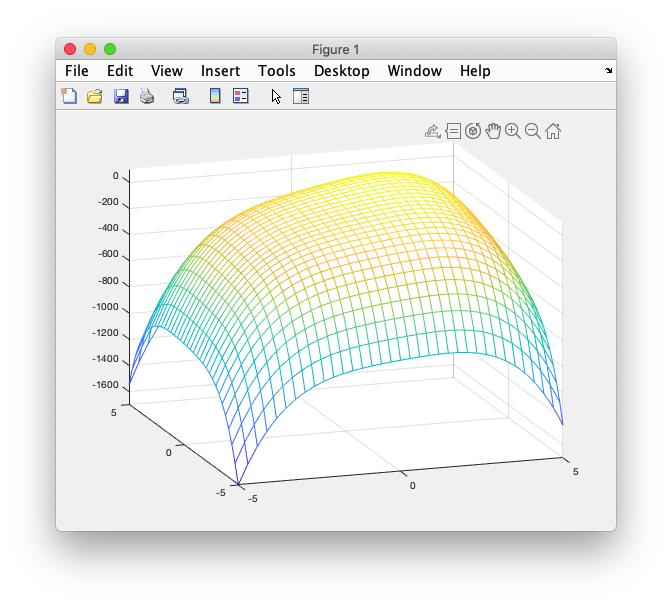
\includegraphics[scale=.4]{images/september2008_1_plot.png}
	\caption{Izris funkcije~\ref{eq:september2008_1} na intervalu $[-5, 5]$.}
	\label{img:september2008_1_plot}
\end{figure}
Iz grafa je razvidno, da imamo opravka z 1 globalnim maksimumom, ki ga poiščemo s \texttt{fminsearch}. Deifiniramo si funkcijo v ločenem \textit{m-file} (\texttt{september2008\_1.m}):
\lstinputlisting[language=Matlab]{exams/september2008_1.m}
... in pokličemo funkcijo v okolici $[-3, -3]$:
\begin{lstlisting}[language=Matlab]
[x, fval] = fminsearch(@(x)-september2008_1(x), [-3, -3])
% Vrne v stilu:
% x = [1.9548    1.8380]
% fval = -92.6766
\end{lstlisting}
Ne smemo pozabiti, ker smo obrnili predznak za maksimizacijo, je obrnjen tudi predznak vrednosti. Pravilna rešitev je torej pri $x_{max} = [1.9548, 1.8380]$ z vrednostjo $f(x_{max}) = 92.6766$.


\subsubsection{Naloga 2.)}

\textbf{Navodila:} \\ Maksimiziraj funkcijo in izračunaj njeno vrednost v točki maksimuma:
\begin{equation} \label{eq:september2008_2}
	f(x) = -(x_1 - x_2)^2 - (x_3 - 1)^2 - 1 - 0.02(x_1^5 + x_2^5 + x_3^5 - 16)^2
\end{equation}

\textbf{Rešitev:} \\
Funkcija ima preveč dimenzij za risanje, zato kar poskusimo z nekaj sreče. Definiramo si nov \textit{m-file} (\texttt{september2008\_2.m}:
\lstinputlisting[language=Matlab]{exams/september2008_2.m}
... in kličemo funkcijo \texttt{fminsearch} (z obratno vrednostjo ker maksimiziramo):
\lstinputlisting[language=Matlab]{exams/september2008_2_script.m}
Ker smo v tem primeru iskali maksimum funkcije, lahko rezultat sortiramo kar naraščujoče, saj je potrebno spremeniti predznak in je najmanjša vrednost enaka največi.
Vidimo, da je prvih 10 najdenih točk identičnih, torej lahko vzamemo maksimum $x_{max} = [1.4963, 1.4963, 1.0000]$ in vrednost $f_{max} = -1$ (ne pozabimo na $-$).


\subsubsection{Naloga 3.)}

\textbf{Navodila:} \\
Določi minimum funkcije in njeno vrednost v točki minimuma:
\begin{equation} \label{eq:september2008_3}
 	f(x) = 2x_1 +x_2^3 + x_3^2
\end{equation}
ob naslednjih omejitvah:
\begin{equation} \label{con:september2008_3}
	\begin{gathered}
		x_1^2 + 2x_2^2 +x_3^2 \geq 4
		x_1, x_2, x_3 \geq 0
	\end{gathered}
\end{equation}

\textbf{Rešitev:} \\
V ločenih \textit{m-file} si definiramo funkcijo (\texttt{september2008\_3.m}):
\lstinputlisting[language=Matlab]{exams/september2008_3.m}
... in omejitve (\texttt{september2008\_3\_con.m}):
\lstinputlisting[language=Matlab]{exams/september2008_3_con.m}
... in kličemo funkcijo \texttt{fmincon}:
\begin{lstlisting}
[x, fval, flag] = fmincon(@(x)september2008_3(x), [1 1 1], [], [], [], [], zeros(1, 3), [], @(x)september2008_3_con(x))
% Vrne v stilu:
%  x = [0.0000    1.3333    0.6667]
%  fval = 2.8148
%  flag = 1
\end{lstlisting}
Matrike $A, b, A_{eq}, B_{eq}$ smo pustili prazne, dodali smo spodnjo mejo ničel, zgornjo mejo nedefinirano in podali omejitve v ločenem \textit{m-file}.
Pridobljena rešitev je očitno veljavna (\texttt{flag = 1}): $x_{min} = [0.0000, 1.3333, 0.6667]$, vrednost pa je $f(x_{min}) = 2.8148$.


\subsection{Izpit 19. Januar 2012}

\subsubsection{Naloga 3.)}

Narisemo si skico. (Slika na namizju)
Imamo dva podobna trikotnika, narisemo si kote in uporabimo kotne funkcije da racunamo l1 + l2 = l. Funkcijo racunamo kot minimum ??? Ker ce racunamo maksimum dobimo resitev neskoncno.
Resitev naloge je f = 7.621m, $\alpha = 0.7482 RAD$



\subsubsection{Naloga 4.)}

Startamo v 1 in hocemo prit v 9. Povezave so usmerjene, lahko gres le v doloceno smer (ni negativnih povezav). Nastavit je treba neke enacbe. Lahko imamo spremenljivke vozlisca, druga moznost pa je da so spremenljivke povezave. Tu je logicno da je spremenljivka povezave. Iz vsakega vozlisca se lahko odlocimo da gremo po eni poti ali ne. Torej 1 -> 2 povezava (recimo ji x(1)) pove ali smo sli po poti (=1) ali ne (=0).

Nastavit moramo nek sistem enacb. Spremenljivke bomo oznacevali z $x_{vhod, izhod}$.
Ker v x1 zacnemo je prva omejitev:
$x_12 + x_13 + x_14 = 1$ // <- tocno po eni izmed poti mormo
Podnobna enacba dobimo za zadnje vozlisce
$x_79 + x_69 + x_89 = 1$ // <- tocno po eni povezavi moramo prit v sink

Podobne enacbe moramo spisat za vas vmesna vozlisca.
Recimo za vozlisce st. 3:
vsota prihodnih mora bit enaka vsoti izhodnih (ce smo prisli v neko vozlisce potem moramo iz njega tudi oditi)
$x_25 + x_35 = x_56 + x_57 + x_{58}$

treba je prestet vse puscice pa prestevilcit spremenljivke -> x1, x2, x3, x4 ... x16
A, b sta prazni -> vse omejitve so tipa je enako
Aeq ima 16 stolpcev in 9 vrstic -> pri 7 so desne strani 0, pri source pa sink pa je desna stran 1


\subsection{Izpit 10. februar 2014}

Izpit je profesor pokazal na vajah.

\subsubsection{Naloga 1.)}
\label{task:feb2014_1}

\textbf{Navodila:} \\
Poišči vsaj dvajset različnih globalnih minimumov funkcije in njihovo vrednost (vse so enake) v teh točkah.
\footnotesize
\begin{equation}
f(x) = \left( \sum_{i=1}^{5}i\cos((i + 1)x_1 + i) \right)\left( \sum_{i=1}^{5}i\cos((i + 1)x_2 + i) \right) \left( \sum_{i=1}^{5}i\cos((i + 1)x_3 + i) \right) 
 \left( \sum_{i=1}^{5}i\cos((i + 1)x_4 + i) \right)
\end{equation}
\normalsize
in omejitvijo spremenljivk $-10 \leq x_i \leq 10$. \\

\noindent POMOČ: Ker bo ročno iskanje minimumov z različnimi starnimi točkami preveč zamudno, si lahko pomagaš s kratkim programčkom za iskanje najoljših rešitev!
Po elektronski pošti oddaj tudi vse izdelane programe in dobljene rešitve!

\vspace{5mm}
\noindent \textbf{Rešitev:} \\
Definiramo si funkcijo v novem \textit{m-file} (\texttt{februar2014\_1\_script.m}):
\lstinputlisting[language=Matlab]{exams/februar2014_1.m}
... in pomožno skripto, ki požene iskanje nad naključno generiranim vhodom. Meje naključnega generiranja postavimo v omejitev, ki je omenjena v navodilih.
\lstinputlisting[language=Matlab]{exams/februar2014_1_script.m}
Po končanem klicu skripte se nam v spremenljivko \texttt{resitve} shranijo vse veljavne vrednosti, v našem primeru je to 100 vrstic (število ponovitev zanke).


\subsubsection{Naloga 2.)}
\label{task:februar2014_2}

\textbf{Navodila:} \\
Poišči maksimum\footnote{V originalnem izpitu je bilo navodilo iskanje minimuma, na vajah je profesor omenil, da je ta problem trivialen in je popravil navodila, da se išče maksimum} podane funkcije in njeno vrednost v tej točki ob navedenih omejitvah za $n=2,3,4,5$.
\begin{equation} 
f(x) = \big( \sqrt{n} \big)^{n} \prod_{i=1}^n x_i
\end{equation}
\begin{equation}
\begin{gathered}
	\sum_{i=1}^n x_i^2 = 1 \\
	0 \leq x_i \leq 1 \quad i=1, ..., n
\end{gathered}
\end{equation}
\textbf{Rešitev:} \\
Kreiramo si nov \textit{m-file} z definicijo funkcije (\texttt{februar2014\_2.m}):
\lstinputlisting[language=Matlab]{exams/februar2014_2.m}
... datoteko z omejitvami (\texttt{februar2014\_2\_con.m}):
\lstinputlisting[language=Matlab]{exams/februar2014_2_con.m}
... in vse skupaj poženemo v nekem skriptu
\lstinputlisting[language=Matlab]{exams/februar2014_2_skript.m}
V skriptu upoštevamo omejitev z naključnim generiranjem med 0 in 1, prvo pa smo eksplicitno zapisali v omejitvah (\texttt{ceq}). V skriptu spreminjamo $n$ vrednost
in dobimo rezultate zanje.

\subsubsection{Naloga 3.)}
\label{task:februar2014_3}

\textbf{Navodila:} \\
Iz lesene krogle s polmerom $10\si{\cm}$ želimo s pomočjo obrezovanja izdelati prisekani stožec, ki bo imel čim večjo možno prostornino (volumen). Koliko bosta znašala polmera osnovnih ploskev takega prisekanega stožca in koliko njegova višina, da bo volumen dobljenega prisekanega stožca maksimalen? Poskusi rešiti nalogo še za minimalni volumen prisekanega stožca, če želimo, da je vsota obeh polmerov osnovnih ploskev v prisekanem stožcu večja kot $12\si{\cm}$.\\
POMOČ: Volumen prisekanega stožca se izračuna po enačbi:
\begin{equation*}
V = \frac{\pi h}{3} \left( R_1^2 + R_2^2 + R_1R_2 \right),
\end{equation*}
kjer sta $R_1$ in $R_2$ polmera osnovnik ploskev prisekanega stožca, $h$ pa njegova višina.

\vspace{5mm} 
\noindent \textbf{Rešitev:} \\
Za takšne geometrijske naloge si je najbolje narisati skico (glej sliko~\ref{img:februar2014_3_sketch}).  
\begin{figure}[hb]
	\centering	
	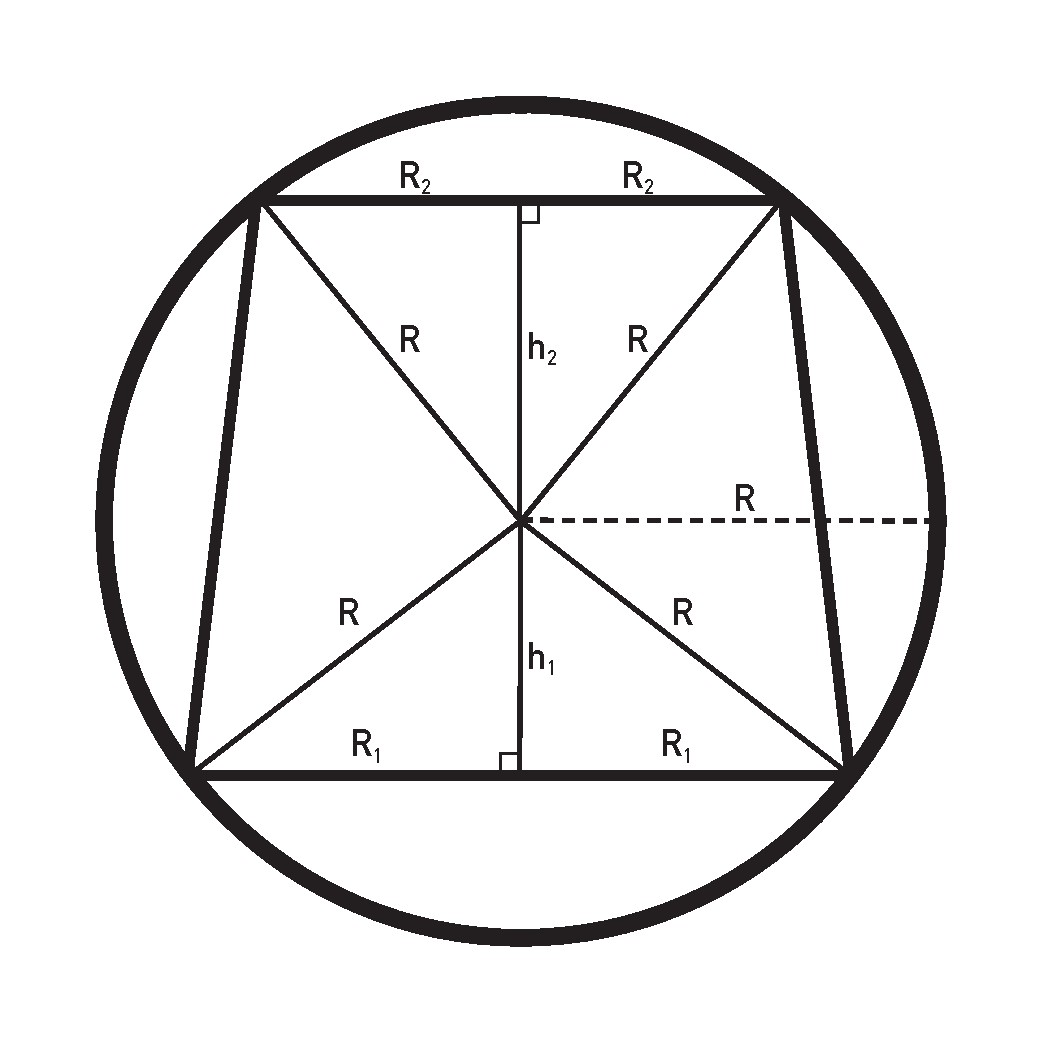
\includegraphics[scale=0.45]{images/februar2014_3_sketch.pdf}
	\caption{Skica z oznakami stranic za pogled iz strani na prisekani stožec vstavljen v kroglo.}
	\label{img:februar2014_3_sketch}
\end{figure}
Iz skice lahko opazimo, da lahko stožec razstavimo na pravokotne trikotnike ($\bigtriangleup R_1 R h_1$ in $\bigtriangleup R_2 R h_2$). Ker je polmer krogle ($R$) podan, bodo naše spremenljivke očitno ($R_1$, $R_2$, $h_1$ in $h_2$). Omejitve lahko zapišemo s pomočjo Pitagorovega izreka:
\begin{equation} \label{con:februar2014_3}
	\begin{gathered}
		R_1^2 + h_1^2 = R^2 \\
		R_2^2 + h_2^2 = R^2 \\
		R_1 + R_2 > 12\si{\cm} $ *$
	\end{gathered}
\end{equation}
To zadnjo omejitev uporabimo le v drugem delu naloge (iskanje najmanjšega stožca, kjer še to drži) in jo v prvem delu izpustimo. Uporabili bomo funkcijo \texttt{fmincon}, zato si definiramo nov \textit{m-file} za definicijo funkcije (\texttt{februar2014\_3.m}):
\lstinputlisting[language=Matlab]{exams/februar2014_3.m}
... in ločenega za definicijo omejitev (\texttt{februar2014\_3\_con.m}):
\lstinputlisting[language=Matlab]{exams/februar2014_3_con.m}
Paziti je treba, da prvotne omejitve~\ref{con:februar2014_3} v Matlabu pretvorimo v ustrezno obliko (vse morajo biti tipa $\leq$ in na desni strani želimo 0).
Kar sledi je še iskanje maksimuma (prvi del naloge):
\begin{lstlisting}[language=Matlab]
[x, fval, flag] = fmincon(@(x)-februar2014\_3(x), [8 7 9 8], [], [], [], [], zeros(1,4), [10 10 10 10], @(x)februar2014\_3\_con(x))
% Vrne:
% x = 5.7735    5.7735    8.1650    8.1650
% fval = -2.4184e+03
% flag = 1
\end{lstlisting}
Ne smemo pozabiti na minus pri definiciji funkcije, začetno točko izberemo naključno, $A$, $b$, $A_{eq}$ in $b_{eq}$ pustimo prazne, za spodnjo omejitev postavimo 0, za zgornjo lahko dodamo desetice (stožec ne sme presegati krogle), vstavimo pa še omejitve $c$ in $c_{eq}$. Rešitev je potemtakem $h_1 = h_2 = 5.7735$ in $R_1 = R_2 = 8.1650$, kar pomeni da največji prisekan stožec je očitno valj.

Da rešimo drugi del naloge (najmanjši volumen ob omejitvi skupnega premera ploskev stožca), pustimo omejitev 3 v $c$ in zopet poženemo \texttt{fmincon}:
\begin{lstlisting}[language=Matlab]
[x, fval, flag] = fmincon(@(x)februar2014_3(x), [5 5 9 1], [], [], [], [], zeros(1,4), [10 10 10 10], @(x)februar2014_3_con(x))
% Vrne:
% x = 0.0000    9.7980   10.0000    2.0000
% fval = 1.2723e+03
% flag = 1
\end{lstlisting}
Klic je enak kot prej, razlika je da tokrat izpustimo minus in malce preuredimo začetno točko (da ne presežemo Matlabovih omejitev pri iskanju). Dobimo še drugo rešitev: $h_1 = 0$, $h_2 = 9.798$, $R_1=10$ in $R_2=2$.


\subsubsection{Naloga 4.)}

\textbf{Navodila:} \\
lastnik tovorjnjaka, ki ima nosilnost tovora 21 ton, ima zahteve po prevozu od štirih podjetij, da bi prepeljal njihove izdelke iz kraja A na kraj B. Vsaka firma
lahko dobavi toliko kosov svojih izdelkov, kot jih je prevoznik pripravljen prepeljati. Izdelki so nedeljivi (morajo biti prepeljani v celih kosih), tabela podaja
teže izdelkov posameznih podjetij in ceno za prevoz enega izdelka. Koliko kosov izdelka posameznega podjetja naj prevoznik sprejme, da bo maksimiziral
svoj zaslužek pri prevozu in tem ne bo presegel nosilnosti tovornjaka? (Nastavi enačbe za reševanje naloge s pomočjo linearnega celoštevilčnega programa in 
ga reši! Oddaj tudi enačbe in opiši pomen posameznih spremenljivk!)

\begin{table} \centering
\begin{tabular}{ | l | p{3cm} | p{3cm} |}
\hline
Podjetje & Teža izdelka v tonah na kos & Prevozni stošek v EUR na kos  \\
\hline
1 & 1 & 13 \\
\hline
2 & 2 & 27 \\
\hline
3 & 3 & 41 \\
\hline
4 & 4 & 55 \\
\hline
\end{tabular}
\end{table}

\vspace{5mm} \noindent \textbf{Rešitev:} \\
Opisan problem spada v kategorijo ILP. Opravka bomo imeli torej z \texttt{intlinprog}. Nastavimo si najprej enačbe. Maksimizirati želimo dobiček, zato je cenitvena funkcija:
\begin{equation*}
f(x) = 13x_1 + 27x_2 + 41x_3 + 55x_4,
\end{equation*}
pri čemer $x_i$ predstavlja količino kupljenega izdelka $i$. Omejitve so nosilnost tovornjaka, prepeljemo lahko le cele izdelke (nedeljivost) in ne moremo prepeljati negativno količino:
\begin{equation*}
\begin{gathered}
1x_1 + 2x_2 + 3x_3 + 4x_4 \leq 21 \\
x_1, x_2, x_3, x_4 \geq 0 \\
x_1, x_2, x_3, x_4 \in \mathbb{N}^0  \\
\end{gathered}
\end{equation*}
Za rešitev v MATLAB ne rabimo posenih skript, lahko si samo definiramo f, A, b, in intcon:
\lstinputlisting[language=Matlab]{exams/februar2014_4.m}
Dobimo maksimalni zaslužek 288 (nasprotna vrednost, zaradi maksimiziranja) pri količinah $x_1 = 1$ in $x_4=5$.
     

\subsection{4. november 2015}

\subsubsection{Naloga 4.}

\textbf{Navodila:}\\
Odvetniška pisarna je sprejela pet novih primerov. Vsakega od primerov lahko rešuje katerikoli izmed petih pravnikov zaposlenih v tej pisarni, a bodo predvidoma
potrebovali različno število ur za njihovo rešitev. Tabela podaja ocene potrebnega števila ur za posameznega pravnika pri posameznem primeru:
\begin{table}[hbt] \centering
\begin{tabular}{| l | c | c | c | c | c |}
\hline 
 & Primer 1 & Primer 2 & Primer 3 & Primer 4 & Primer 5 \\
 \hline
 Pravnik 1 & 145 & 122 & 130 & 95 & 110 \\
 \hline
 Pravnik 2 & 80 & 63 & 85 & 68 & 78 \\
 \hline
 Pravnik 3 & 121 & 107 & 93 & 69 & 95 \\
 \hline
 Pravnik 4 & 118 & 93 & 116 & 80 & 105 \\
 \hline
 Pravnik 5 & 117 & 85 & 120 & 80 & 111 \\
 \hline
\end{tabular}
\end{table}
Določi optimalno prireditev primerov posameznim pravnikom, tako da dobi vsak pravnik drug primer in da je skupno število predvidevih porabljenih ur minimalno. Pomagaj si z linearnim programom.

\vspace{5mm} \noindent \textbf{Rešitev:} \\
Definirajmo si najprej spremenljivke. Ker bomo minimirali število porabljenih ur in lahko vsak pravnik rešuje le enega izmed primerov, si izberemo binarne spremenljivke (imajo vrednost 0 ali 1): 
\begin{center}
$x_1$ ... pravnik 1 rešuje primer 1 \\
$x_2$ ... pravnik 1 rešuje primer 2 \\
... \\
$x_6$ ... pravnik 2 rešuje primer 1 \\
... \\
$x_{25}$ ... pravnik 5 rešuje primer 5 \\
\end{center}
Cenitvena funkcija (minimiziranje ur) postane tako:
\begin{multline}
f(x) = 145x_1 + 122x_2 + 130x_3 + 95x_4 + 110x_5 + \\
+  80x_6 + 63x_7 + 85x_8 + 68x_9 + 78x_{10} +\\
+  121x_{11} + 107x_{12} + 93x_{13} 69x_{14} + 95x_{15} + \\
+ 118x_{16} + 93x_{17} + 116x_{18} + 80x_{19} + 105x_{20} + \\
+ 117x_{21} + 85x_{22} + 120x_{23} + 80x_{24} + 111x_{25} 
\end{multline}
Omejitve pa je potrebno zapisati tako, da vsaka vrstica v zgornji tabeli vrne seštevek 1 in prav tako vsak stolpec!
\begin{equation*}
\begin{gathered}
\sum_{i=1}^5 x_i = 1 $,   $ \sum_{i=6}^{10} x_i = 1 $,   $ \sum_{i=11}^{15} x_i = 1 $,   $ \sum_{i=16}^{20} x_i = 1 $,   $ \sum_{i=21}^{25} x_i = 1 \\
x_1 + x_6 + x_{11} + x_{16} + x_{21} = 1 \\
...
\end{gathered}
\end{equation*}
Zgoraj so zapisane omejitve za vse vrstice in primer omejitve za prvi stolpec. Omejitve za preostale 4 stolpce niso zapisane, so pa upoštevane v kodi v nadaljevanju.

Za rešitev je potrebno definirati matriko $A_{eq}$ in vektor $b_{eq}$, poženemo pa intlinprog: 
\lstinputlisting[language=Matlab]{exams/november2015_4.m}
Rešitev pride 448 porabljenih ur in pravnik 1 rešuje primer 5, pravnik 2 rešuje primer 1, pravnik 3 rešuje primer 3, pravnik 4 rešuje primer 4 in pravnik 5 rešuje primer 2.

\subsection{Poskusni kolokvij 2020}

\subsubsection{Naloga 1.}

Glej nalogo~\ref{task:feb2014_1}

\subsubsection{Naloga 2.}

Glej nalogo~\ref{task:februar2014_2}

\subsubsection{Naloga 3.}

Glej nalogo~\ref{task:februar2014_3}

\subsubsection{Naloga 4.}

Napiši funkcijo \texttt{[x fval] = najkrajsa\_pot(c, i, j)}, ki poišče najkrajšo pot med vozliščema $i$ in $j$ grafa, če je v matriki $c$ podan seznam cen povezav, vrednost $c_{ij}$ je cena poti iz vozlišča $i$ v vozlišče $j$. Funkcija bo vrnila matriko $x$ dimenzije $n\times n$, kjer bo za vsako spremenljivko z 1 ali 0 označeno, če se ta veja nahaja v optimalni poti od vozlišča $i$ do vozlišča $j$, fval pa bo najnižja cena (vsota označenih povezav).

Namig: Znotraj svoje funkcije lahko uporabiš klic MATLAB-ove funkcije \texttt{intlinprog}, podatke za klic pa moraš znotraj svoje funkcije v tem primeru pravilno pripraviti (spremenljivke $f$, $A$, $b$, ...).

Nato s pomočjo napisane funkcije poišči rešitev za najkrajši poti med vozliščema 2 in 7 ter med vozliščema 6 in 1. Uporabi cene povezav iz spodaj podane matrike $c$:

\begin{table}[hbt] \centering
\begin{tabular}{| c |  c |  c |  c |  c |  c |  c |  c | }
\hline
Izvor\textbackslash Cilj & 1 & 2 & 3 & 4 & 5 & 6 & 7 \\
\hline
1 & 1000 & 24 & 9 & 13 & 8 & 36 & 4 \\
\hline
2 & 9 & 1000 & 12 & 3 & 31 & 7 & 75 \\
\hline
3 & 12 & 16 & 1000 & 11 & 5 & 9 & 23 \\
\hline
4 & 20 & 43 & 3 & 1000 & 22 & 18 & 21 \\
\hline
5 & 2 & 18 & 6 & 39 & 1000 & 18 & 13 \\
\hline
6 & 82 & 5 & 1 & 12 & 26 & 1000 & 7 \\
\hline
7 & 45 & 27 & 14 & 37 & 8 & 17 & 1000 \\
\hline
\end{tabular}
\end{table}

\vspace{5mm} \noindent \textbf{Rešitev:}
Za rešitev tega problema si rabimo najprej definirati spremenljivke. Naj bodo to binarne odločitvene spremenljivke, ki povedo ali smo šli po povezavi iz vozlišča ki pripada vrstici v vozlišče, ki pripada stolpcu. Tako dobimo $n^2$ spremenljivk. Cenitvena funkcija naj bo kar matrika zložena v vektor po vrsticah. Torej če gremo po povezavi $e_{ij}$, bo cena takšnega potovanja $c_{ij}$. Vozlišči izvora in ponora morata imeti po en prihod oziroma odhod, zato ti omejitvi pišemo ločeno. Ostale vrstice (za vsako vozlišče po ena) pa imajo odhod enak prihodu ($omejitev_{ij}$ mora biti enaka $omejitev_{ji}$). Ostale posebnosti v kodi so le spreminjanje dimenzij vektorjev in matrik:
\lstinputlisting[language=Matlab]{exams/najkrajsa_pot.m}
Vse skupaj pa lahko poženemo s:
\lstinputlisting[language=Matlab]{exams/poskusni2020_4.m}


\subsection{Neuvrščene}

\subsubsection{Maksimalni pretok v grafu}

\textbf{Navodila:} \\
Podan imamo usmerjen graf, na katerem želimo izračunati največji možen pretok iz izvora $A$ v ponor $D$. Povezave so dvosmerne, vendar lahko po eni povezavi peljemo le toliko kolikor je označeno na povezavah (primer: $A$ v $B$ sprejme 10, $B$ v $A$ pa 0). (Namig: v kolikor ni podano v navodilih, da je potrebno pridobiti rešitev s pomočjo linearnega programa, lahko uporabimo MATLAB \texttt{graph} ali \texttt{digraph} in funkcijo \texttt{maxflow}).

\begin{figure}[hbt]
	\centering
	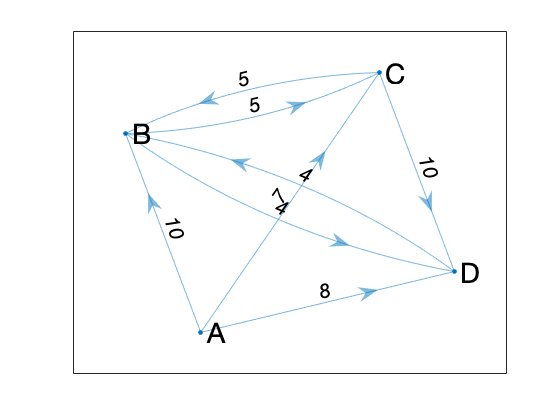
\includegraphics[width=0.5\textwidth]{images/unlisted1_graph.png}
	\caption{Graf povezav. V kolikor povezava ni označena na grafu pomeni, da po njej ne moremo peljati toka (ima utež 0).}
	\label{img:unlisted1_graph}
\end{figure}

\vspace{5mm} \noindent \textbf{Rešitev:}\\
Označimo si najprej spremenljivke na grafu:
\begin{equation*}
\begin{gathered}
A \rightarrow B ... x_ 1 \\
A \rightarrow C ... x_2 \\
A \rightarrow D ... x_3 \\
B \rightarrow C ... x_4 \\
B \rightarrow D ... x_5 \\
C \rightarrow B ... x_6 \\
D \rightarrow B ... \text{ ignoriramo, ker iz ponora ne želimo vzeti toka} \\
C \rightarrow D ... x_7 
\end{gathered}
\end{equation*}
Naslednji korak je spisati cenitveno funkcijo. Maksimizirati želimo tok ki priteče v ponor, torej želimo maksimizirati tok, ki teče po povezavah katerih cilj je ponor:
\begin{equation*}
f(x) = x_3 + x_5 + x_7
\end{equation*}
Omejitve je potrebno definirati tako, da lahko iz vozlišča odteče le toliko toka kolikor ga je na voljo (vozlišče $A$ - izvor ima na voljo neskončno veliko toka):
\begin{equation*}
\begin{gathered}
x_1 + x_6 = x_4 + x_5 \\
x_2 + x_4 = x_6 + x_7 
\end{gathered}
\end{equation*}
Prva omejitev je za vozlišče $B$, na levi strani so povezave, ki pripeljejo tok, na desni pa tiste ki ga odpeljejo. Druga omejitev je spisana po istem načinu za vozlišče $C$.  Seveda je potrebno omejitve spraviti v MATLAB obliko (vse na levo stran in $\leq$ ali $=$).

Spišemo precej enostaven program, paziti je le potrebno na predznak funkcije ker maksimiziramo:
\lstinputlisting[language=Matlab]{exams/unlisted1_graph.m}
Prišli smo do rešitve, maksimalen pretok je 22, x pa vsebuje koliko toka smo prepeljali po vsaki povezavi

\subsubsection{Transportni problem}

Imamo Rent-a-Car ponudnika, ki ima dva vira (skladišča) avtomobilov. Na prvem ima parkiranih 15 avtov, na drugem pa 13. Imajo tudi 4 poslovalnice (cilji), pri katerih si stranke lahko izposojajo avtomobile. Predvidevajo, da potrebujejo na na cilju 1 9 avtov, na cilju 2 6 avtov, na cilju 3 7 avtov in na cilju 4 9 avtov. Opazimo, da je zaloge avtomobilov manj, imamo pa tudi stroške da pripeljemo avto iz skladišča v poslovalnico:
\begin{table}[hbt] \centering
\begin{tabular}{|c |c | c | c | c |}
\hline
	Vir \textbackslash Cilj  & 1 & 2 & 3 & 4 \\
\hline	
	1  & 45 & 17 & 21 & 30 \\
\hline	
	2  & 14 & 18 & 19 & 31 \\
\hline
\end{tabular}
\end{table}
Z upoštevanjem potreb poslovalnic po avtomobilih in stroškov, da prepeljemo avtomobil iz enega izmed skladišč najdite najcenejšo rešitev prevažanja avtomobilov.

\vspace{5mm} \noindent \textbf{Rešitev:} \\
Želimo minimizirati stroške prevoza, zato bodo naše spremenljivke koliko avtov smo pripeljali iz katerega skladišča v katero poslovalnico. Definirajmo torej $x_1$ je število avtomobilov pripeljanih iz vira 1 v cilj 1, $x_2$ je količina avtomobilov pripeljanih iz vira 1 v cilj 2, ... in $x_8$ je količina avtomobilov pripeljanih iz vira 2 v cilj 4. Naša cenitvena funkcija tako postane:
\begin{equation*}
f(x) = 45x_1 + 17x_2 +21x_3 + 30x_4 + 14x_5 + 18x_6 + 19x_7 + 31x_8
\end{equation*} 
Prvi omejitvi sta količini avtov na vsakem izmed virov:
\begin{equation*}
\begin{gathered}
x_1 + x_2 + x_3 + x_4 = 15 \\
x_5 + x_6 + x_7 + x_8 = 13
\end{gathered}
\end{equation*}
Pomemben je predznak $=$, saj imamo premalo zalogo. Ker minimiziramo stroške pa upoštevamo tudi potrebe na ciljih (po nepotrebnem ne prevažamo avtov):
\begin{equation*}
\begin{gathered}
x_1 + x_5 \leq 9 \\
x_2 + x_6 \leq 6 \\
x_3 + x_7 \leq 7 \\
x_4 + x_8 \leq 9 \\
\end{gathered}
\end{equation*}
Ker imamo zaloge manj kot je potrebe moramo paziti na predznak $\leq$. V kolikor bi imeli dovolj zaloge ali pa preveč, bi lahko uporabili predznak $=$. Manjkajo še omejitve nenegativnosti in pa celoštevilčnosti (polovica avta na enem cilju in polovica na drugem nam ne koristi).

Uporabimo MATLAB in \texttt{intlinprog}:
\lstinputlisting[language=Matlab]{exams/unlisted_car_rental.m}
Najcenejši strošek je torej 547, uporabili pa smo 9 avtov iz vira 2 na cilj 1, 6 avtov iz vira 1 na cilj 2, 3 avte iz vira 1 na cilj 3, 4 avte iz vira 2 na cilj 3 in 6 avtov iz vira 1 na cilj 4.


\subsubsection{Graf problem}

(slika na namizju graf\_problem.png) Kombiniran problem dostave izdelkov. Imamo 6 transportnih vozlisc. Stevilke na vozliscih (+ pomeni da je toliko izdelkov v tem skladisci na zalogi), ciljna vozlisca pa so tista kjer je minus (koliko izdelkov rabi). Oznake na povezavah pomenijo ceno za transport enega izdelka po tej povezavi. Cilj naloge je poiskati najcenejso varianto da pripeljemo potrebne kolicine izdelkov iz skladisc v sink (iz + vozlisc v - vozlisca). Vozlisce 4 je vmesno vozlisce, pomeni da ni ne skladisce in ne ponor - preko njega se samo peljemo.

Problem je podoben najkrajse poti in maks flow, s tem da je to vse skombinirano skupaj. Najprej si spet definiramo spremenljivke (katera povezava je katera spremenljivka)
1->2 .. x1
1->3 .. x2
1->4 .. x3
3->2 .. x4
3->4 .. x5
4->2 .. x6
4->6 .. x7
4->5 .. x8
5->6 .. x9
2->6 .. x10
Cenitvena funkcija f:
f = [5 3 3 14 10 3 8 6 15 4];


Ker imamo dovolj zaloge (70 zloage, potrebujemo 60) lahko uporabimo enacaje -> v primeru da ni dovolj zaloge uporabimo $\leq$
Enacba za ciljno vozlisce 2
x1 + x4 + x6 - x10 = 25   Aeq
Enacba za ciljno vozlisce 6
x7 + x9 +x10 = 35  Aeq

Za vsa vozlisca je treba napisati taksne enacbe
Enacba za vozlisce 3
x2 + 20 >= x4 + x5 ... lahko kaj ostane v zalogi (na levi strani), ker je imamo vec, zato damo $\geq$  A
Enacba vozlisce 4 (odhodne povezave smo premaknili na levo stran))
x3 + x5 + x8 - x6  - x7 = 0  Aeq
Enacba vozlisce 5  
x8 + x9 <= 30  A
Enacba za vozlisce 1
x1 + x2 + x3 <= 20  A


A = [ 0 -1 0 1 1  0 0 0 0 0; 0 0 0 0 0 0 0 1 1 0; 1 1 1 0 0 0 0 0 0 0]
b = [20; 30; 20]
Aeq = [1 0 0 1 0 1 0 0  0 -1; 0 0 0 0 0 0 1 0 1 1;  0 0 1 0 1 -1 -1 1 0 0] .. 1 in -1 so odvisne ker das enacbe na isto stran in znak mora biti vseposod $\leq$
beq = [25; 35; 0]
LB = zeros(1,10)
UB  .. je prazen (ne vemo neke dobre omejitve)
vse resitve zelimo celostevilcne
[x, fval] = intlinprog(f, ones(1,9), A, b, Aeq, beq, LB)
f* = 640
x* = [20 0 0 0 10 40 0 30 0 35]


\subsubsection{Geometrijska naloga}

Slika na namizju (skica-geometrijska.png)
Posici dolzini diagonal tako, da bo ploscina stirikotnika s podanimi stranicami maksimalna. Nato posici se dolzini diaognal za min ploscino stirikotnika ob dodanih pogojih (e <= c+d-0.5, f < a+d-0.5). Koliko znasata maksimalna in minimalna ploscina?

Bretschneider's formula -> katerokili stirikotnik ... obstaja bolj preprost nacin
Razdelis ga na 2 trikotnika -> ABD in BCD, pa sestavis ploscino iz dveh trikotnikov (Heron's formula) (v splosnem -> S = sqrt( s(s-a)(s-b)(s-c) ), pri cemer je s = (a+b+c)/2)

S = S1 + S2 = sqrt( s1 (s1-a) (s1-f) (s1-d))  + sqrt(s2 (s2-b) (s2-c) (s2-x))
s1 = (a + d + x) / 2
s2 = (b + c + x) / 2	... spremenili smo f v x
kriterijska funkcija 
f = S1 + S2
Omejitve: trikotniska neenakost
x < 13 (a+d || b+c) -> lahko kar recemo UB = 13 (malo manj ko 13)

Maksimum	x=9.33 cm, S = 40.9878 cm2
					y = 8.896 cm (diagonala e) ... ploscino sestavis iz drugih dveh trikotnikov (naceloma dobis isto ploscino, ali pa iz 2 stranic zracunas drugo diagonalo)
					
Minimum ima dodatne omejitve -> lik razpade ce ne bi blo dodatnih omejitev (manjka se pogoj konkavnosti ... recimo noben notranji kot ne sme bit > $\pi$). 
konveksen lik:
	S=36.5591 x=11.1399, y=10.5
konkavni lik (se ni iskalo, se pa lahko naredi (ena diagonala je zunaj lika)
	S=11.7264, x=3.1, y=?? 


\subsubsection{Graf maksimalna neodvisna mnozica (barvanje)}

Imamo nek graf (maks-neodvisna-mnozica.png). Iskalne maksimalne neodvisne mnozice: Zelimo dolocena vozlisca pobarvat z 1 eno barvo -> tako da niti dve pobarvani vozlisci nista sosedi (med pobarvanima vozliscema ne sme biti direktne povezave).
Lahko se lotis z linearnim programiranjem, hevristiko, evolucijski algoritmi ... ali pa SAT Solver (Boolovi izrazi -> ce so vsi true potem si nasel resitev, das na vsako povezavo da ne sme bit source in sink pobarvana).


\end{document}
